\section{Spans}

Let $\vect{u}$ and $\vect{v}$ be two non-parallel vectors in
$\R^n$. We can picture the set of their linear combinations as follows:
\begin{center}
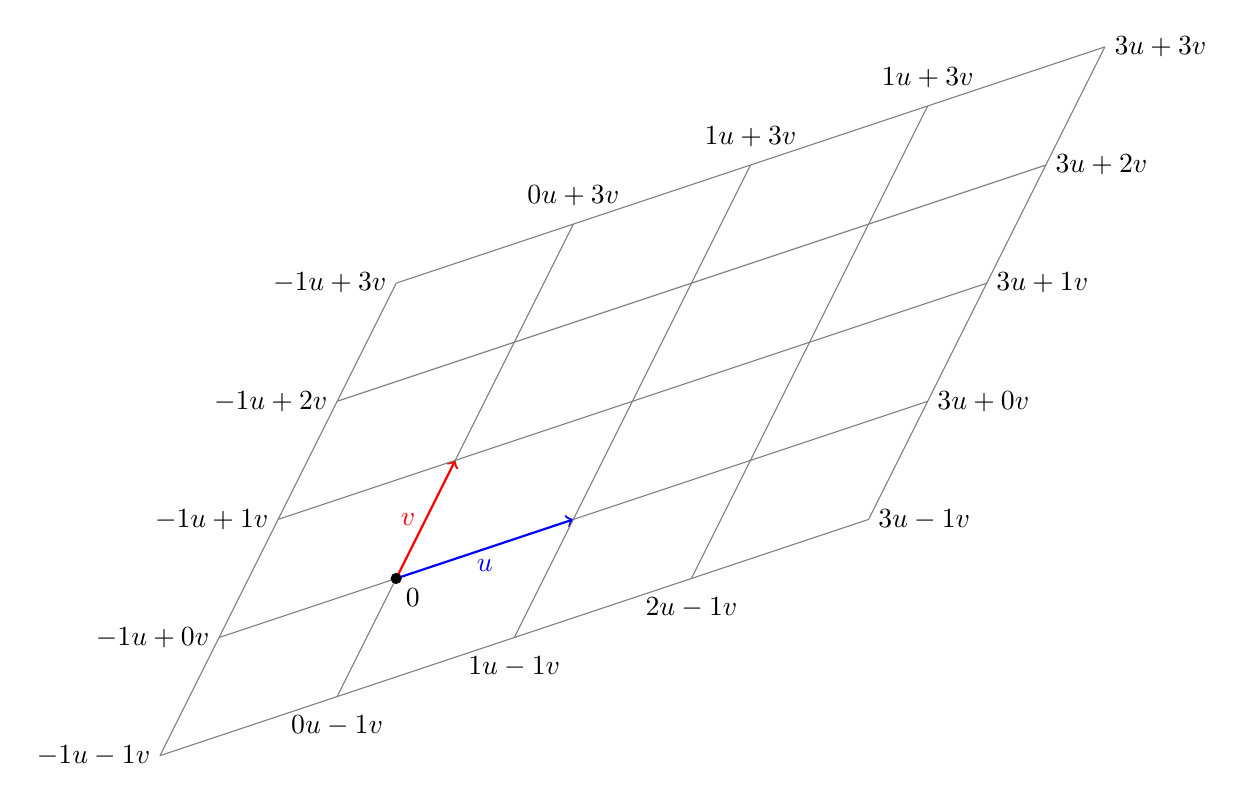
\begin{tikzpicture}[scale=1.5]
\draw[->, thick, blue] (0,0) -- node[below]{$\vect{u}$} (1.5,0.5);
\draw[->, thick, red] (0,0) -- node[left]{$\vect{v}$} (0.5,1);
\draw[-, gray] (-2,-1.5)--(4,0.5);
\draw[-, gray] (-1.5,-0.5)--(0,0);
\draw[-, gray] (1.5,0.5)--(4.5,1.5);
\draw[-, gray] (-1,0.5)--(5,2.5);
\draw[-, gray] (-0.5,1.5)--(5.5,3.5);
\draw[-, gray] (0,2.5)--(6,4.5);
\draw[-, gray] (-2,-1.5)--(0,2.5);
\draw[-, gray] (-0.5,-1)--(0,0);
\draw[-, gray] (0.5,1)--(1.5,3);
\draw[-, gray] (1,-0.5)--(3,3.5);
\draw[-, gray] (2.5,0)--(4.5,4);
\draw[-, gray] (4,0.5)--(6,4.5);
\draw (-2.0,-1.5) node[left]{$-1\vect{u}-1\vect{v}$};
\draw (-1.5,-0.5) node[left]{$-1\vect{u}+0\vect{v}$};
\draw (-1.0,0.5) node[left]{$-1\vect{u}+1\vect{v}$};
\draw (-0.5,1.5) node[left]{$-1\vect{u}+2\vect{v}$};
\draw (0.0,2.5) node[left]{$-1\vect{u}+3\vect{v}$};
\draw (1.5,3.0) node[above=0.75ex]{$0\vect{u}+3\vect{v}$};
\draw (3.0,3.5) node[above=0.75ex]{$1\vect{u}+3\vect{v}$};
\draw (4.5,4.0) node[above=0.75ex]{$1\vect{u}+3\vect{v}$};
\draw (6.0,4.5) node[right]{$3\vect{u}+3\vect{v}$};
\draw (5.5,3.5) node[right]{$3\vect{u}+2\vect{v}$};
\draw (5.0,2.5) node[right]{$3\vect{u}+1\vect{v}$};
\draw (4.5,1.5) node[right]{$3\vect{u}+0\vect{v}$};
\draw (4.0,0.5) node[right]{$3\vect{u}-1\vect{v}$};
\draw (2.5,0.0) node[below=0.75ex]{$2\vect{u}-1\vect{v}$};
\draw (1.0,-0.5) node[below=0.75ex]{$1\vect{u}-1\vect{v}$};
\draw (-0.5,-1.0) node[below=0.75ex]{$0\vect{u}-1\vect{v}$};
\draw[fill] (0,0) circle [radius=1.2pt] node[below right]{$\vect{0}$};
\end{tikzpicture}
\end{center}
As the picture shows, the linear combinations of $\vect{u}$ and
$\vect{v}$ form a 2-dimensional plane through the origin. We say that
this plane is \textbf{spanned}\index{span}\index{vector!span} by the
vectors $\vect{u}$ and $\vect{v}$.  This concept generalizes to more
than two vectors. For example, three vectors may span a 3-dimensional
space (although sometimes, they span only a 2-dimensional space, or
even a line). This motivates the following definition.

\begin{definition}{Span of a set of vectors}{span}
  The set of all linear combinations of the vectors
  $\vect{u}_1, \ldots ,\vect{u}_k$ in $\R^{n}$ is known as the
  \textbf{span}\index{span}\index{vector!span} of these vectors and is written
  as $\sspan\set{\vect{u}_1,\ldots,\vect{u}_k}$. Using set notation,
  we can write
  \begin{equation*}
    \sspan\set{\vect{u}_1,\ldots,\vect{u}_k}
    ~=~ \set{a_1\vect{u}_1+\ldots+a_k\vect{u}_k \mid a_1,\ldots,a_k\in\R}.
  \end{equation*}
\end{definition}

\begin{example}{Vectors in a span}{vector-in-span}
  Let $\vect{u}=\begin{mymatrix}{r} 1 \\ 1 \\ 1 \end{mymatrix}$ and
  $\vect{v}=\begin{mymatrix}{r} 3 \\ 2 \\ 1 \end{mymatrix}$. Which
  of the following vectors are elements of
  $\sspan\set{\vect{u},\vect{v}}$?
  \begin{equation*}
    (a)\quad\vect{w} = \begin{mymatrix}{r} 2 \\ 3 \\ 4 \end{mymatrix},
    \qquad
    (b)\quad\vect{z} = \begin{mymatrix}{r} 1 \\ 1 \\ 2 \end{mymatrix}.
  \end{equation*}
\end{example}

\begin{solution}
  (a) For a vector to be in $\sspan\set{\vect{u},\vect{v}}$, it must
  be a linear combination of $\vect{u}$ and $\vect{v}$. Therefore,
  $\vect{w}\in\sspan\set{\vect{u},\vect{v}}$ if and only if we can
  find find scalars $a,b$ such that
  $a\,\vect{u} + b\,\vect{v} = \vect{w}$. We must therefore solve the
  equation
  \begin{equation*}
    a \begin{mymatrix}{r} 1 \\ 1 \\ 1 \end{mymatrix}
    + b \begin{mymatrix}{r} 3 \\ 2 \\ 1 \end{mymatrix}
    = \begin{mymatrix}{r} 2 \\ 3 \\ 4 \end{mymatrix}.
  \end{equation*}
  We write this as an augmented matrix and solve. 
  \begin{equation*}
    \begin{mymatrix}{rr|r}
      1 & 3 & 2 \\
      1 & 2 & 3 \\
      1 & 1 & 4 \\
    \end{mymatrix}
    \sim\ldots\sim
    \begin{mymatrix}{rr|r}
      1 & 0 & 5 \\
      0 & 1 & -1 \\
      0 & 0 & 0 \\
    \end{mymatrix}.
  \end{equation*}
  The solution is $a=5$ and $b=-1$. This means that
  $\vect{w} = 5\vect{u} + (-1)\vect{v}$. Therefore, $\vect{w}$ is an
  element of $\sspan\set{\vect{u},\vect{v}}$.

  (b) We repeat the same method with the vector $\vect{z}$. This time,
  we have to find $a,b$ such that
  $a\,\vect{u} + b\,\vect{v} = \vect{z}$. The system of equations is
  \begin{equation*}
    \begin{mymatrix}{rr|r}
      1 & 3 & 1 \\
      1 & 2 & 1 \\
      1 & 1 & 2 \\
    \end{mymatrix}
    \sim\ldots\sim
    \begin{mymatrix}{rr|r}
      1 & 3 & 1 \\
      0 & -1 & 0 \\
      0 & 0 & 1 \\
    \end{mymatrix},
  \end{equation*}
  which is inconsistent. Therefore, there is no solution. We conclude
  that $\vect{z}$ is not an element of
  $\sspan\set{\vect{u},\vect{v}}$.
\end{solution}

\begin{example}{Describing the span}{describe-span}
  Describe the span of the vectors
  $\vect{u}=\begin{mymatrix}{r} 1 \\ 1 \\ 1 \end{mymatrix}$ and
  $\vect{v}=\begin{mymatrix}{r} 3 \\ 2 \\ 1 \end{mymatrix}$ in
  $\R^{3}$.
\end{example}

\begin{solution}
  Let $\vect{w} = \mat{x, y, z}^T$ be any vector. Proceeding as in the
  previous example, we know that $\vect{w}$ is an element of
  $\sspan\set{\vect{u},\vect{v}}$ if and only if the equation
  \begin{equation*}
    a \begin{mymatrix}{r} 1 \\ 1 \\ 1 \end{mymatrix}
    + b \begin{mymatrix}{r} 3 \\ 2 \\ 1 \end{mymatrix}
    = \begin{mymatrix}{r} x \\ y \\ z \end{mymatrix}
  \end{equation*}
  is consistent. Note that the variables of this equation are $a,b$;
  we regard $x,y,z$ as constants for the moment. We write the augmented
  matrix of this system and reduce to {\ef}:
  \begin{equation*}
    \begin{mymatrix}{rr|c}
      1 & 3 & x \\
      1 & 2 & y \\
      1 & 1 & z \\
    \end{mymatrix}
    \stackrel{R_2\leftarrow R_2-R_1}{\stackrel{R_2\leftarrow R_3-R_1}{\sim}}
    \begin{mymatrix}{rr|c}
      1 & 3 & x \\
      0 & -1 & y-x \\
      0 & -2 & z-x \\
    \end{mymatrix}
    \stackrel{R_3\leftarrow R_3-2R_2}{\sim}
    \begin{mymatrix}{rr|c}
      1 & 3 & x \\
      0 & -1 & y-x \\
      0 & 0 & (z-x)-2(y-x) \\
    \end{mymatrix},
  \end{equation*}
  From the {\ef}, we see that the system is consistent if and only if
  $(z-x)-2(y-x)=0$, or equivalently $x - 2y + z = 0$. Therefore, the
  vector $\vect{w}$ is in $\sspan\set{\vect{u},\vect{v}}$ if and only
  if $x - 2y + z = 0$. In other words, the span of $\vect{u}$ and
  $\vect{v}$ is the plane $x - 2y + z = 0$.
\end{solution}

\begin{example}{Span of redundant vectors}{redundant-span}
  Let $\vect{u}=\begin{mymatrix}{r} 1 \\ 1 \\ 1 \end{mymatrix}$,
  $\vect{v}=\begin{mymatrix}{r} 3 \\ 2 \\ 1 \end{mymatrix}$, and
  $\vect{w}=\begin{mymatrix}{r} 11 \\ 8 \\ 5 \end{mymatrix}$.
  Show that
  $\sspan\set{\vect{u},\vect{v},\vect{w}} =
  \sspan\set{\vect{u},\vect{v}}$.
\end{example}

\begin{solution}
  Observe that $\vect{w} = 2\,\vect{u}+3\,\vect{v}$. Therefore,
  $\vect{w}$ is already in the span of $\vect{u}$ and $\vect{v}$.  Two
  sets are equal if they have the same elements, i.e., each element of
  the first set is an element of the second set and vice
  versa. Therefore, to show
  $\sspan\set{\vect{u},\vect{v},\vect{w}} =
  \sspan\set{\vect{u},\vect{v}}$, we must show (a) that every element
  of $\sspan\set{\vect{u},\vect{v},\vect{w}}$ is an element of
  $\sspan\set{\vect{u},\vect{v}}$ and (b) vice versa.

  (a) Let $\vect{z}$ be an arbitrary element of
  $\sspan\set{\vect{u},\vect{v},\vect{w}}$. Then, by definition of
  span, there exist scalars $a,b,c$ such that
  \begin{eqnarray*}
    \vect{z} &=& a\,\vect{u} + b\,\vect{v} + c\,\vect{w}.
  \end{eqnarray*}
  But as observed above, we have $\vect{w} = 2\,\vect{u}+3\,\vect{v}$,
  and therefore we can also write
  \begin{eqnarray*}
    \vect{z}
    &=& a\,\vect{u} + b\,\vect{v} + c(2\,\vect{u}+3\,\vect{v})\\
    &=& (a+2c)\vect{u} + (b+3c)\vect{v}.
  \end{eqnarray*}
  It follows that $\vect{z}$ is a linear combination of $\vect{u}$ and
  $\vect{v}$, and therefore, $\vect{z}\in \sspan\set{\vect{u},\vect{v}}$. 

  (b) Clearly every linear combination of $\vect{u}$ and $\vect{v}$ is
  also a linear combination of $\vect{u}$, $\vect{v}$, and $\vect{w}$,
  namely, taking the coefficient of $\vect{w}$ to be $0$. Therefore,
  every element of $\sspan\set{\vect{u},\vect{v}}$ is an element of
  $\sspan\set{\vect{u},\vect{v},\vect{w}}$.

  Because we have shown that every element of
  $\sspan\set{\vect{u},\vect{v},\vect{w}}$ is an element of
  $\sspan\set{\vect{u},\vect{v}}$ and vice versa, it follows that
  $\sspan\set{\vect{u},\vect{v},\vect{w}}$ and
  $\sspan\set{\vect{u},\vect{v}}$ are the same set of vectors.
\end{solution}

In the situation of the last example, we say that the vector
$\vect{w}$ is \textbf{redundant}%
\index{redundant vector}\index{vector!redundant}; it does not
contribute anything to
$\sspan\set{\vect{u},\vect{v},\vect{w}}$. Geometrically, the three
vectors $\vect{u}$, $\vect{v}$, and $\vect{w}$ lie in a plane. Since
the two vectors $\vect{u}$ and $\vect{v}$ are sufficient to span this
plane, the third vector $\vect{w}$ is not really needed. We will study
this situation more systematically in the next section. 

\begin{example}{Span of the empty set}{span-empty-set}
  We talked about the span of $k$ vectors
  $\vect{u}_1,\ldots,\vect{u}_k$.  What if $k=0$? What is
  the span of an empty set of vectors? 
\end{example}

\begin{solution}
  Consider what happens when we compute the sum of three numbers. We
  usually write this as $b_1+b_2+b_3$. We can also compute the sum of
  three numbers by starting from $0$ and then adding each of the three
  numbers to it. I.e., the sum can be computed as
  $0+b_1+b_2+b_3$. Similarly, we can write the sum of two numbers as
  $0+b_1+b_2$, and the sum of just one number as $0+b_1$. Continuing
  the pattern, it follows that the sum of zero numbers should be $0$:
  \begin{center}
    \begin{tabular}{ll}
      Sum of 3 numbers: & $0+b_1+b_2+b_3$. \\
      Sum of 2 numbers: & $0+b_1+b_2$. \\
      Sum of 1 numbers: & $0+b_1$. \\
      Sum of 0 numbers: & $0$. \\
    \end{tabular}
  \end{center}
  The sum of zero numbers is also called the \textbf{empty sum}%
  \index{empty sum}. It is equal to the unit of addition, i.e., $0$.
  By an analogous argument, the empty sum of vectors is equal to the
  unit of vector addition, i.e., to the zero vector $\vect{0}$%
  \index{zero vector}\index{vector!zero vector}.  In general, if we
  have $k$ vectors $\vect{u}_1,\ldots,\vect{u}_k$, the span consists
  of all vectors of the form $a_1\vect{u}_1+\ldots+a_k\vect{u}_k$,
  which is a sum of $k$ vectors.  In case $k=0$, the span consists
  only of the empty sum, i.e., the zero vector $\vect{0}$, which we
  also call the \textbf{empty linear combination}%
  \index{empty linear combination}%
  \index{vector!empty linear combination}%
  \index{linear combination!empty}. Therefore, the span of the empty
  set of vectors is $\set{\vect{0}}$.
\end{solution}
